\documentclass{beamer}

\usepackage{beamerthemesplit}
\usepackage[utf8x]{inputenc}
\usepackage{pgf}
\usepackage{default}
\usepackage{url}
\usepackage{subfigure}
\usepackage{algorithmic} 
\usepackage{algorithm} 
\usepackage{amssymb}
\usepackage{graphicx}
\usepackage{booktabs}

\usetheme{Singapore}


%Define some commands for printing correct variables in math mode 
\newcommand{\av}{\textbf{a}}
\newcommand{\bv}{\textbf{b}}
\newcommand{\cv}{\textbf{c}}
\newcommand{\dv}{\textbf{d}}
\newcommand{\ev}{\textbf{e}}
\newcommand{\fv}{\textbf{f}}
\newcommand{\gv}{\textbf{g}}
\newcommand{\hv}{\textbf{h}}
\newcommand{\iv}{\textbf{i}}
\newcommand{\jv}{\textbf{j}}
\newcommand{\kv}{\textbf{k}}
\newcommand{\lv}{\textbf{l}}
\newcommand{\mv}{\textbf{m}}
\newcommand{\nv}{\textbf{n}}
\newcommand{\ov}{\textbf{o}}
\newcommand{\pv}{\textbf{p}}
\newcommand{\qv}{\textbf{q}}
\newcommand{\rv}{\textbf{r}}
\newcommand{\sv}{\textbf{s}}
\newcommand{\tv}{\textbf{t}}
\newcommand{\uv}{\textbf{u}}
\newcommand{\vv}{\textbf{v}}
\newcommand{\wv}{\textbf{w}}
\newcommand{\xv}{\textbf{x}}
\newcommand{\yv}{\textbf{y}}
\newcommand{\zv}{\textbf{z}}

\newcommand{\alphav}{\mbox{\boldmath$\alpha$}}
\newcommand{\betav}{\mbox{\boldmath$\beta$}}
\newcommand{\gammav}{\mbox{\boldmath$\gamma$}}
\newcommand{\xiv }{\mbox{\boldmath$\xi$}}
\newcommand{\muv}{\mbox{\boldmath$\mu$}}
\newcommand{\tauv}{\mbox{\boldmath$\tau$}}
\newcommand{\Omegam}{\mbox{\boldmath$\Omega$}}
\newcommand{\Lambdam}{\mbox{\boldmath$\Lambda$}}
\newcommand{\Sigmam}{\mbox{\boldmath$\Sigma$}}
\newcommand{\Gammam}{\mbox{\boldmath$\Gamma$}}
\newcommand{\Deltam}{\mbox{\boldmath$\Delta$}}
\newcommand{\Thetam}{\mbox{\boldmath$\Theta$}}
\newcommand{\Phim}{\mbox{\boldmath$\Phi$}}
\newcommand{\Pim}{\mbox{\boldmath$\Pi$}}

\newcommand{\diag}{\mbox{diag}}
\newcommand{\tr}{\mbox{tr}}
\newcommand{\card}{\mbox{card}}
\newcommand{\cov}{\mbox{cov}}
\newcommand{\sign}{\mbox{sign}}
\newcommand{\var}{\mbox{var}}
\newcommand{\st}{\mbox{s.t.}}
\newcommand{\rank}{\mbox{rank}}
\newcommand{\argmin}{\mbox{argmin}}
\newcommand{\argmax}{\mbox{argmax}}

\newcommand{\Am}{\textbf{A}}
\newcommand{\Bm}{\textbf{B}}
\newcommand{\Cm}{\textbf{C}}
\newcommand{\Dm}{\textbf{D}}
\newcommand{\Em}{\textbf{E}}
\newcommand{\Fm}{\textbf{F}}
\newcommand{\Gm}{\textbf{G}}
\newcommand{\Hm}{\textbf{H}}
\newcommand{\Imat}{\textbf{I}}
\newcommand{\Jm}{\textbf{J}}
\newcommand{\Km}{\textbf{K}}
\newcommand{\Lm}{\textbf{L}}
\newcommand{\Mm}{\textbf{M}}
\newcommand{\Nm}{\textbf{N}}
\newcommand{\Om}{\textbf{O}}
\newcommand{\Pm}{\textbf{P}}
\newcommand{\Qm}{\textbf{Q}}
\newcommand{\Rm}{\textbf{R}}
\newcommand{\Sm}{\textbf{S}}
\newcommand{\Tm}{\textbf{T}}
\newcommand{\Um}{\textbf{U}}
\newcommand{\Vm}{\textbf{V}}
\newcommand{\Wm}{\textbf{W}}
\newcommand{\Xm}{\textbf{X}}
\newcommand{\Ym}{\textbf{Y}}
\newcommand{\Zm}{\textbf{Z}}

%Use regular expression: (\[a-z])([^a-zA-Z])  -> \1v\2  to change old style macros 
\graphicspath{{./Figures/}}

\title{Statistics and the Analysis of Data\\ Lecture 2: Multivariate Data}
\author{Charanpal Dhanjal \\ \texttt{charanpal@gmail.com}} 
\institute{\'{E}cole des Ponts}
\date{\today}

\begin{document}

\frame{\titlepage}

\begin{frame}{Recap Part I}  
\begin{itemize} 
 \item Started with observations $n$ variables $x_1, \ldots, x_n$ 
 \item Histograms 
 \begin{itemize}
   \item Discrete case: $h(x) = \sum_{i=1}^n \mathcal{I}(x_i = x)$
 \item Continuous: \emph{bins} $ I_1, \ldots, I_k$, $n_j = \sum_{x_i} \mathcal{I}\{x_i \in I_j\}$
 \end{itemize} 
 \item Cumulative distribution function: $F(x) = \frac{1}{n}\sum_{i=1}^n \mathcal{I}(x_i \leq x)$
 \item Averages - mean, mode, median 
 \item Dispersion 
 \begin{itemize}
 \item $var(x) = \frac{1}{n}\sum_{i=1}^n (x_i - \bar{x})^2$
 \item Standard deviation, mean absolute deviation
 \item Interquartile range
 \end{itemize}
\end{itemize}
\end{frame}

\begin{frame}{Recap Part II}  
 \begin{itemize} 
  \item Order quantiles: $q_\alpha^x$ in which $x_{(m)}$ and $m = \lceil \alpha n \rceil$
  \item Box plot: 
  \begin{itemize} 
  \item Bounded by $(A, Q1, med(x), Q3, B)$ 
  \end{itemize}
  \item Paired samples: $x_1, \ldots, x_n$ and $y_1, \ldots, y_n$. 
   \begin{itemize}
   \item Covariance, correlation 
   \item Scatter plot 
   \item Linear regression 
   \item QQPlots: plot $q_\alpha^x$ and $q_\alpha^y$
   \end{itemize}
  \end{itemize}
\end{frame}

\begin{frame}{Overview} 
\begin{itemize} 
 \item Looked at $\{x_1, \ldots, x_n\} \in \mathbb{R}$ and then paired variables $\{(x_1, y_1), \ldots, (x_n, y_n)\} \in \mathbb{R}^2$
\item Natural extension: $\{(x_{11}, \ldots, x_{1d}) \ldots, (x_{n1}, \ldots, x_{nd})\} \in \mathbb{R}^d$
\item Represent in matrix form 
\begin{displaymath} 
 \textbf{X} = \left[\begin{array}{c c c} x_{11} & \ldots & x_{1d} \\ 
                     \vdots & \ddots & \vdots \\
 x_{n1} & \ldots & x_{nd}  \end{array} \right] 
\end{displaymath}
\item How can we study data like this? 
 \end{itemize}
\end{frame}

\begin{frame}{Introduction}
\begin{itemize} 
 \item Scatter plots are hard when $d > 3$ 
 \item If \emph{features} (columns) of $\textbf{X}$, denoted $\textbf{X}_{(i)}$, are independent can easily study them 
 \item In practice, dependencies (correlations) may exist
  \begin{itemize}
    \item Want to cut out those features
    \end{itemize}
    \item One solution: Principal Components Analysis (PCA)
\end{itemize}
\end{frame}

\begin{frame}{Running Example: Banknote Authentication} 
\begin{itemize}
 \item Features represent properties about genuine and forged banknote-like specimens
 \item Computed upon images of notes 
 \begin{itemize}
  \item Variance of wavelet transformed features, skewness, kurtosis, entropy 
  \item 4 features in total 
  \item 1372 observations 
 \end{itemize}
 \item Want to understand how these features predict forgeries 
\end{itemize}
\end{frame}

\begin{frame}{Initial Analysis} 
\begin{itemize} 
 \item First, study correlations of pairs of variables
\end{itemize}

\begin{table}
\centering
\resizebox{\linewidth}{!} {% 
\begin{tabular}{l | l l l l}
 & $\textbf{X}_{(1)}$ & $\textbf{X}_{(2)}$ & $\textbf{X}_{(3)}$ & $\textbf{X}_{(4)}$ \\ 
 \hline
$\textbf{X}_{(1)}$ & 1.000 & 0.264 & -0.381 & 0.277\\
$\textbf{X}_{(2)}$ & 0.264 & 1.000 & -0.787 & -0.526\\
$\textbf{X}_{(3)}$ & -0.381 & -0.787 & 1.000 & 0.319\\
$\textbf{X}_{(4)}$ & 0.277 & -0.526 & 0.319 & 1.000\\
\end{tabular} }
\end{table} 
\begin{itemize} 
 \item $\textbf{X}_{(2)}$ and $\textbf{X}_{(3)}$ are correlated (skewness, kurtosis)
 \item $\textbf{X}_{(2)}$ and $\textbf{X}_{(4)}$ are correlated (skewness, entropy)
\end{itemize}
\end{frame}

\begin{frame}{Principal Components Analysis (PCA)} 
\begin{itemize} 
 \item Could use other forms of analysis (e.g. scatter plots in 3D, box plots) 
 \item Limited to 3 dimensions 
 \item PCA can work with \emph{any} dimension $\geq 1$
 \begin{itemize} 
 \item The idea is to form a linear combination of columns of $\textbf{X}$ that are uncorrelated 
 \item Call the output variables $\textbf{Z}_{(1)}, \ldots, \textbf{Z}_{(k)}$, $k \leq d$
 \item In some sense the $k$ new features carry useful information 
 \end{itemize}
\end{itemize}
\end{frame}

\begin{frame}{Some Notations}
\begin{itemize} 
 \item Observations are now column vectors in $\mathbb{R}^d$
 \item Some properties 
 \begin{itemize}
 \item Inner product 
 \begin{displaymath} 
  \langle \uv, \vv \rangle = \uv^T\vv = \sum_{i=1}^d \uv_i \vv_i
 \end{displaymath}
 \item Norm 
 \begin{displaymath} 
  \|\uv\|^2 = \sum_{i=1}^d \uv_i^2 = \langle \uv, \uv \rangle
 \end{displaymath}
 \end{itemize} 
 \item Identity matrix $\Imat$
\end{itemize}
\end{frame}


\begin{frame}{Preprocessing} 
\begin{itemize} 
 \item PCA works best with centered data: 
 \begin{displaymath} 
  \xv \leftarrow \xv - \bar{\xv}, \quad  \bar{\xv} = \frac{1}{n}\sum_{i=1}^n \xv_i
 \end{displaymath}
\item Must also normalise the range of each feature to have unit variance 
\begin{displaymath}
 \xv \leftarrow \frac{\xv}{\sqrt{\var(\xv)}}, \quad \var(\xv) = \frac{1}{n}\sum_{i=1}^n \|\xv_i - \bar{\xv}\|^2
\end{displaymath}

\item From now on, assume observations are centered and normalised 
\end{itemize}
\end{frame}

\begin{frame}{Exercise}
\begin{itemize} 
 \item Write down an expression for the variance of a set of centered observations. 
 \item Let $\xv_1, \ldots, \xv_n$ be a set of observations such that $\bar{\xv} \neq 0$ and denote $\zv_i = \xv_i - \bar{\xv}$. Show the relationship between the variance of $\xv$ and $\yv$. 
\end{itemize}
 
\end{frame}


\begin{frame}{Total Variance} 
\begin{itemize} 
 \item Study the total variance of a set of observations (called \emph{inertia})
 \item $I(\Xm) = \sum_{i=1}^d \|\Xm_{(i)}\|^2 = p$
 \item Can segment $d$ dimensional space using projections onto an \emph{orthogonal matrix} $\Vm \in \mathbb{R}^{d \times k}$ 
 \begin{itemize}
  \item Orthogonal means $\Vm^T\Vm = \Imat$ i.e. columns of $\Vm$ are perpendicular to each other
 \end{itemize}
\end{itemize}
\end{frame}

\begin{frame}{Subspace Projection}
\begin{itemize} 
 \item Partition of space using $\Vm$ and $\Imat - \Vm$
 \begin{displaymath}
  \sum_{i=1}^n \|\xv_{i}^T\Vm \|^2 + \sum_{i=1}^n \|\xv_{i}^T(\Imat - \Vm)\|^2 = I(\Xm)
 \end{displaymath}
\item Note maximising $\sum_{i=1}^n \|\xv_{i}^T\Vm \|^2 $ is the same as minimising $\sum_{i=1}^n \|\xv_{i}^T(\Imat - \Vm)\|^2$ 
\end{itemize}
\end{frame}

\begin{frame}{Exercise} 
\begin{itemize} 
 \item Show that the following statement is true
  \begin{displaymath}
  \sum_{i=1}^n \|\xv_{i}^T\Vm \|^2 + \sum_{i=1}^n \|\xv_{i}^T(\Imat - \Vm)\|^2 = I(\Xm)
 \end{displaymath}
\end{itemize}
\end{frame}


\begin{frame}{Maximising Variance I}
\begin{itemize}
 \item We want a $k$ dimensional projection that captures most variance such that $\Vm^T\Vm = \Imat$
 \begin{displaymath}
  \max \phi(\Vm) = \max \sum_{i=1}^n \|\xv_{i}^T\Vm \|^2
 \end{displaymath}

\end{itemize}
\end{frame}

\begin{frame} 
\begin{itemize}
 \item Show that 
 \begin{displaymath} 
 \phi(\Vm) = \sum_{i=1}^n \|\xv_{i}^T\Vm \|^2 = \tr(\Vm^T\Xm^T\Xm\Vm) 
 \end{displaymath}
 where $\tr(\Am) = \sum_{i=1}^n \Am_{ii}$
\end{itemize}

\end{frame}


\begin{frame}{Covariance Matrix}
\begin{itemize} 
 \item $\Xm^T\Xm$ is known as the \emph{covariance} matrix 
 \item What are the diagonal elements of this matrix? 
 \item Note that the covariance matrix is symmetric which means $\Am^T = \Am$
\end{itemize}
\end{frame}

\begin{frame}{Maximising Variance II} 
\begin{itemize} 
 \item Can write $\phi(\Vm) = \tr(\Vm^T\Xm^T\Xm\Vm) = \sum_{i=1}^k \vv_i^T\Xm^T\Xm\vv_i$
 \item Therefore can iterate:
 \begin{enumerate}
  \item Initialise $\hat{\Vm} = []$
  \item For $j = 1, \ldots, k$
  \begin{enumerate}
  \item Solve $\vv_j = \argmax \; \vv^T\Xm^T\Xm\vv \quad \st \;  \vv \bot \hat{\Vm}, \|\vv \|  = 1$
  \item Let $\hat{\Vm} \leftarrow [\hat{\Vm} \; \vv_{j}]$
   \end{enumerate}
\item Solution $\Vm = \hat{\Vm}$
 \end{enumerate}
\item How do we find the maximum of $\vv^T\Xm^T\Xm\vv$? 
\end{itemize}
\end{frame}

\begin{frame}{Maximising Variance III}  
\begin{itemize} 
 \item Can write $\Xm^T\Xm = \sum_{i=1}^d \lambda_i \uv_i \uv_i^T$, known as \emph{eigen-decomposition}
  \begin{itemize} 
  \item Eigenvectors are orthogonal and have unit norm and $\lambda_1 \geq \lambda_2 \geq \cdots \geq \lambda_d$ 
  \item We know eigenvalues $\lambda$ are real and non-negative 
  \end{itemize} 
\end{itemize}
\end{frame}

\begin{frame}{Exercise}
\begin{itemize} 
 \item Let $\Xm \in \mathbb{R}^{n \times d}$ and $\Cm = \Xm^T\Xm$. Show that the eigenvalues of $\Cm$ are real and nonnegative. 
\end{itemize}
\end{frame}


\begin{frame}{Maximising Variance IV}  
\begin{itemize}
\item Follows that $\vv^T\Xm^T\Xm\vv = \sum_{i=1}^d \lambda_i (\uv_i^T\vv)^2$
\item Note $(\uv_i^T\vv)^2$ is 1 (its max value) when $\vv = \uv_i$
\begin{itemize}
\item Therefore $\max \; \vv^T\Xm^T\Xm\vv = \lambda_1$ and $\vv_1 = \uv_1$
\end{itemize}
\item To find $\max \; \vv^T\Xm^T\Xm\vv \quad \st \;  \vv \bot \vv_1, \ldots \vv_{j-1}, \|\vv \|  = 1$ we pick $\vv = \vv_{j} = \uv_{j}$
\item The resulting projections $\Xm\vv_1, \ldots, \Xm\vv_k$ are called the \emph{Principal Components} 
\end{itemize}
\end{frame}

\begin{frame}{Exercise}  
\begin{itemize} 
 \item Show that the principal components $\Xm\vv_1, \ldots, \Xm\vv_k$ are orthogonal i.e. $(\Xm\vv_i)^T\Xm\vv_j = 1$ if $i=j$ otherwise $0$ (implies they are uncorrelated)
 \item Show also that the principal components are centered 
\end{itemize}
\end{frame}

\begin{frame}{PCA on banknotes I} 
\begin{itemize}
 \item Compute first 3 principal components 
\end{itemize}
  \begin{figure}[htp]
\mbox{
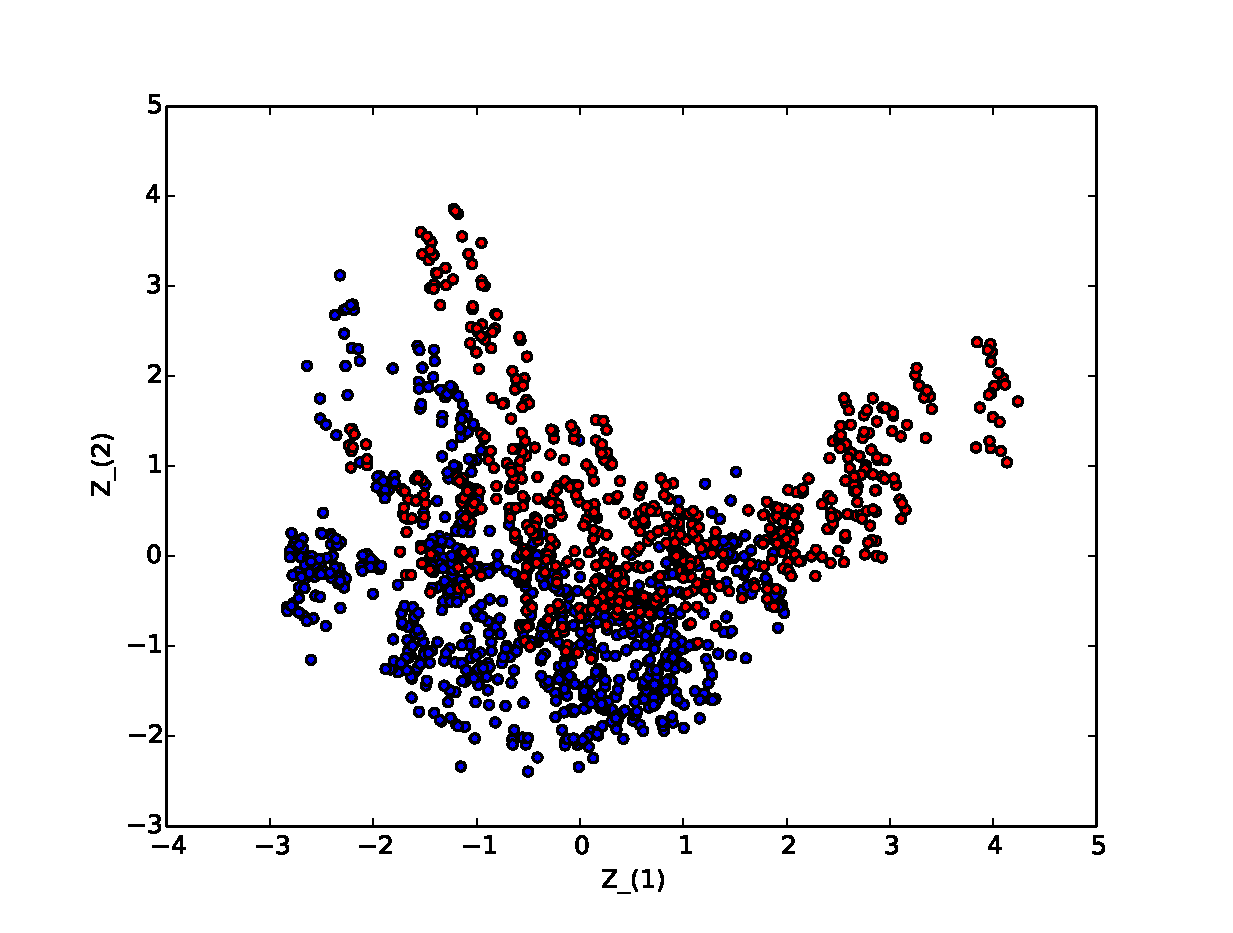
\includegraphics[width=0.5\linewidth]{Z12.eps}
}
\end{figure} 
\end{frame}

\begin{frame}{PCA on banknotes II}
  \begin{figure}[htp]
\mbox{
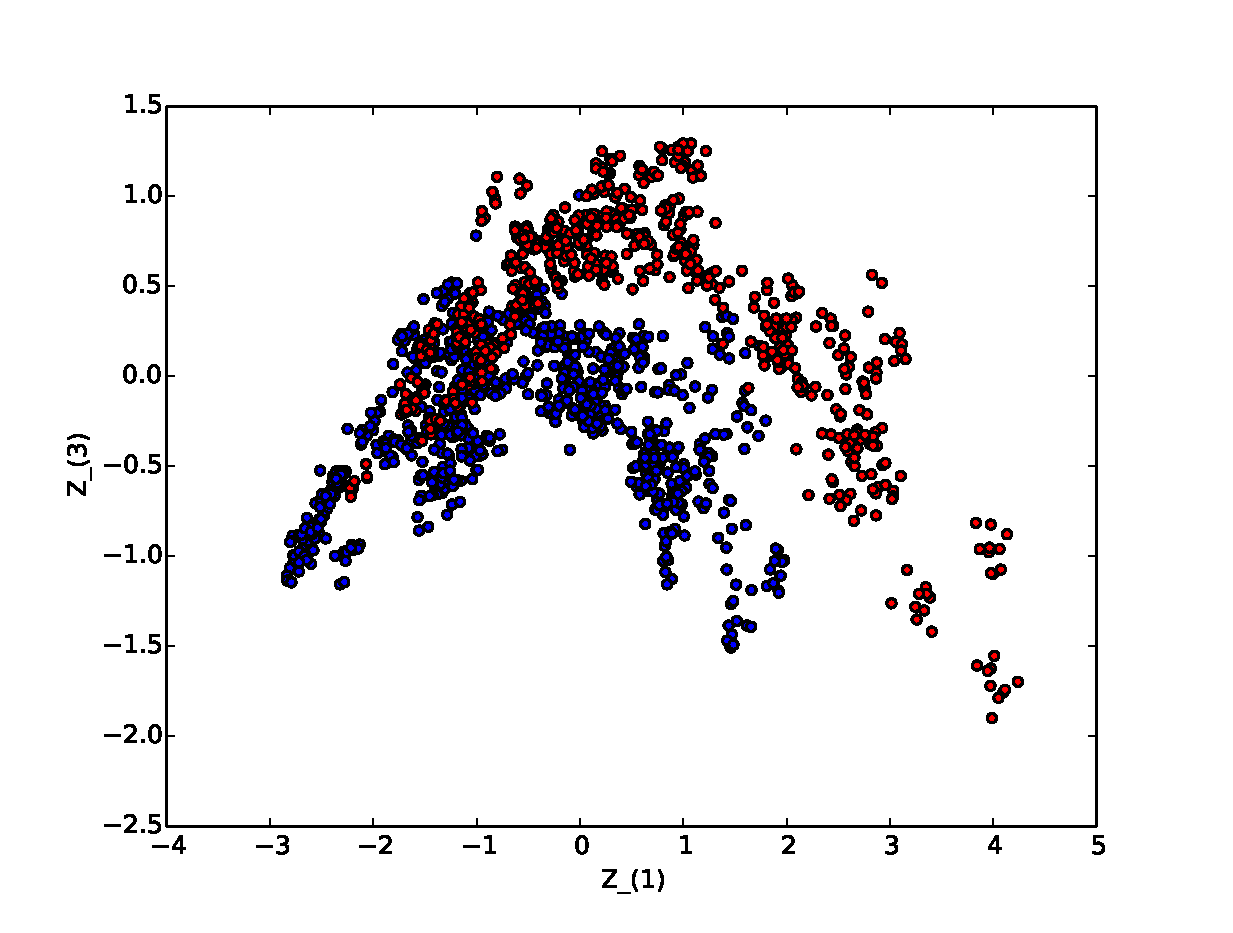
\includegraphics[width=0.5\linewidth]{Z13.eps}
}
\end{figure} 
\end{frame}

\begin{frame}{PCA on banknotes III} 
  \begin{figure}[htp]
\mbox{
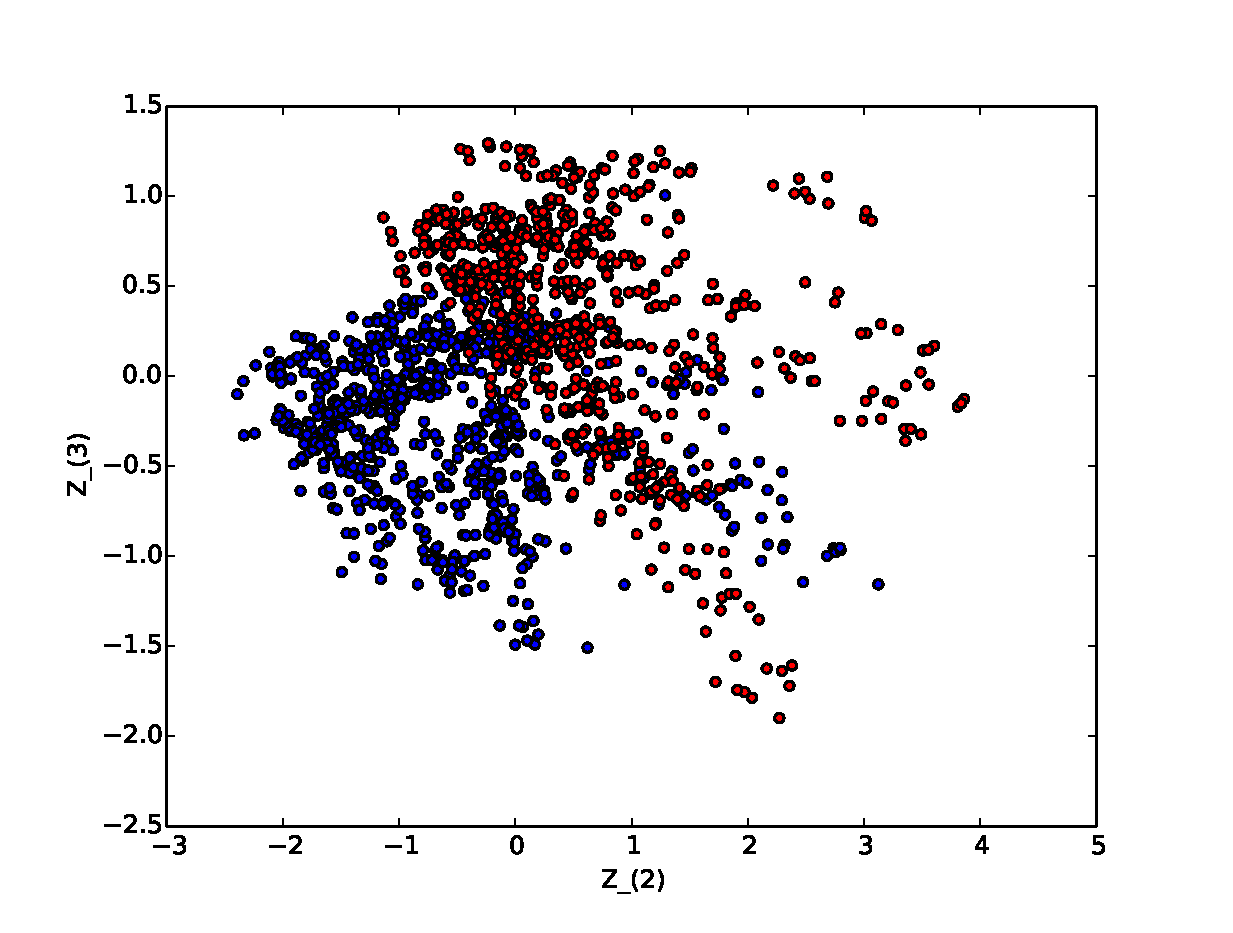
\includegraphics[width=0.5\linewidth]{Z23.eps}
}
\end{figure} 
\begin{itemize}
 \item Can discriminate on these features 
\end{itemize}

\end{frame}

\begin{frame}{Interpretation} 
\begin{itemize} 
 \item First eigenvector is a linear combination of input features 
 \begin{itemize}
  \item Can assign ``importance'' to original features 
  \item First eigenvector: $[-0.249 \quad -0.639 \quad 0.613 \quad 0.392]^T$
 \end{itemize} 
 \item Eigenvalue is variance covered
 \begin{itemize}
  \item We have $0.545,  0.323,  0.088$ covered by 1st 3 eigenvalues 
  \item $~ 0.868$ by first 2 eigenvalues 
  \end{itemize}
\end{itemize} 
\end{frame}

\begin{frame}{An Interesting Metric} 
\begin{itemize} 
 \item Give a particular observation $\xv$ what is the \emph{approximation error} when using $k$ PCs?
 \begin{displaymath} 
  \epsilon(\xv, \Vm) = \|\xv - \Vm^T\Vm^T\xv\|^2
 \end{displaymath}
\item Answer:
\begin{eqnarray*} 
  \|\xv - \Vm^T\Vm^T\xv\|^2 &=& (\xv - \Vm\Vm^T\xv)^T (\xv - \Vm\Vm^T\xv) \\ 
   &=& \xv^T\xv - \xv^T\Vm\Vm^T\xv \\ 
   &=& \|\xv\|^2 - \|\Vm^T\xv\|^2
\end{eqnarray*}
\end{itemize}
\end{frame}

\begin{frame}{Summary} 
\begin{itemize}
 \item Multivariate data is common in practice 
 \item PCA is a way to decorrelate and find useful features that are linear combinations of original features 
 \begin{itemize}
  \item Key idea is find features which maximise variance 
 \end{itemize}
 \item Resulting features can be used for visualisation or discrimination 
\end{itemize}
\end{frame}

\end{document}
